% 这是中国科学院大学计算机科学与技术专业《计算机组成原理(研讨课)》使用的实验报告 Latex 模板
% 本模板与 2024 年 2 月 Jun-xiong Ji 完成, 更改自由 Shing-Ho Lin 和 Jun-Xiong Ji 于 2022 年 9 月共同完成的基础物理实验模板
% 如有任何问题, 请联系: jijunxoing21@mails.ucas.ac.cn
% This is the LaTeX template for report of Experiment of Computer Organization and Design courses, based on its provided Word template. 
% This template is completed on Febrary 2024, based on the joint collabration of Shing-Ho Lin and Junxiong Ji in September 2022. 
% Adding numerous pictures and equations leads to unsatisfying experience in Word. Therefore LaTeX is better. 
% Feel free to contact me via: jijunxoing21@mails.ucas.ac.cn

\documentclass[11pt]{article}

\usepackage[a4paper]{geometry}
\geometry{left=2.0cm,right=2.0cm,top=2.5cm,bottom=2.5cm}

\usepackage{ctex} % 支持中文的LaTeX宏包
\usepackage{amsmath,amsfonts,graphicx,subfigure,amssymb,bm,amsthm,mathrsfs,mathtools,breqn} % 数学公式和符号的宏包集合
\usepackage{algorithm,algorithmicx} % 算法和伪代码
\usepackage[noend]{algpseudocode} % 算法和伪代码
\usepackage{fancyhdr} % 自定义页眉页脚
\usepackage[framemethod=TikZ]{mdframed} % 创建带边框的框架
\usepackage{fontspec} % 字体设置
\usepackage{adjustbox} % 调整盒子大小
\usepackage{fontsize} % 设置字体大小
\usepackage{tikz,xcolor} % 绘制图形和使用颜色
\usepackage{multicol} % 多栏排版
\usepackage{multirow} % 表格中合并单元格
\usepackage{pdfpages} % 插入PDF文件
\usepackage{listings} % 在文档中插入源代码
\usepackage{wrapfig} % 文字绕排图片
\usepackage{bigstrut,multirow,rotating} % 支持在表格中使用特殊命令
\usepackage{booktabs} % 创建美观的表格
\usepackage{circuitikz} % 绘制电路图
\usepackage{zhnumber} % 中文序号(用于标题)
\usepackage{tabularx} % 表格折行

\definecolor{dkgreen}{rgb}{0,0.6,0}
\definecolor{gray}{rgb}{0.5,0.5,0.5}
\definecolor{mauve}{rgb}{0.58,0,0.82}
\lstset{
  frame=tb,
  aboveskip=3mm,
  belowskip=3mm,
  showstringspaces=false,
  columns=flexible,
  framerule=1pt,
  rulecolor=\color{gray!35},
  backgroundcolor=\color{gray!5},
  basicstyle={\small\ttfamily},
  numbers=none,
  numberstyle=\tiny\color{gray},
  keywordstyle=\color{blue},
  commentstyle=\color{dkgreen},
  stringstyle=\color{mauve},
  breaklines=true,
  breakatwhitespace=true,
  tabsize=3,
}

% 轻松引用, 可以用\cref{}指令直接引用, 自动加前缀. 
% 例: 图片label为fig:1
% \cref{fig:1} => Figure.1
% \ref{fig:1}  => 1
\usepackage[capitalize]{cleveref}
% \crefname{section}{Sec.}{Secs.}
\Crefname{section}{Section}{Sections}
\Crefname{table}{Table}{Tables}
\crefname{table}{Table.}{Tabs.}

% \setmainfont{Palatino Linotype.ttf}
% \setCJKmainfont{SimHei.ttf}
% \setCJKsansfont{Songti.ttf}
% \setCJKmonofont{SimSun.ttf}
\punctstyle{kaiming}
% 偏好的几个字体, 可以根据需要自行加入字体ttf文件并调用

\renewcommand{\emph}[1]{\begin{kaishu}#1\end{kaishu}}

% 对 section 等环境的序号使用中文
\renewcommand \thesection{\zhnum{section}、}
\renewcommand \thesubsection{\arabic{section}}


%%%%%%%%%%%%%%%%%%%%%%%%%%%
%改这里可以修改实验报告表头的信息
\newcommand{\name}{艾华春, 李霄宇, 王敬华}
\newcommand{\studentNum}{2022K8009916011,2022K8009929029,2022K8009925009}
\newcommand{\major}{计算机科学与技术}
\newcommand{\labNum}{5}
\newcommand{\labName}{AXI总线接口设计}
%%%%%%%%%%%%%%%%%%%%%%%%%%%

\begin{document}

\begin{center}
  \LARGE \bf 中国科学院大学 \\《计算机体系结构基础(研讨课)》实验报告
\end{center}

\begin{center}
  \emph{姓名} \underline{\makebox[10em][c]{\name}} \\
  % 如果名字比较长, 可以修改box的长度"8em"为其他值
  \emph{学号} \underline{\makebox[30em][c]{\studentNum}}\\
  % \emph{专业} \underline{\makebox[15em][c]{\major}}\\
  \emph{实验项目编号} \underline{\makebox[3em][c]{\labNum}}
  \emph{实验名称} \underline{\makebox[30em][c]{\labName}}\\
\end{center}

% \begin{center}
%   \begin{tabularx}{\textwidth}{|lX|}
%     \hline
%     注1: & 撰写此 Word 格式实验报告后以 PDF 格式保存 SERVE CloudIDE 的 \texttt{/home/serve-ide/ cod-lab/reports} 目录下(注意:reports 全部小写)。文件命名规则:\texttt{prjN.pdf},其中 \texttt{prj} 和后缀名 \texttt{pdf} 为小写,\texttt{N} 为1至4的阿拉伯数字。例如:\texttt{prj1.pdf}。PDF 文件大小应控制在 5MB 以内。此外,实验项目5包含多个选做内容,每个选做实验应提交各自的实验报告文件,文件命名规则:\texttt{prj5-projectname.pdf},其中``-''为英文标点符号的短横线。文件命名举例:\texttt{prj5-dma.pdf}。具体要求详见实验项目5讲义。 \\

%     注2: & 使用\texttt{git add}及\texttt{git commit}命令将实验报告\texttt{PDF}文件添加到本地仓库master分支,并通过\texttt{git push}推送到实验课SERVE GitLab远程仓库master分支(具体命令详见实验报告)。 \\

%     注3: & 实验报告模板下列条目仅供参考,可包含但不限定如下内容。实验报告中无需重复描述讲义中的实验流程。\\
%     \hline
%   \end{tabularx}
% \end{center}

  

\section{逻辑电路结构与仿真波形的截图及说明}
\noindent
$\bullet$
\textbf{取值模块添加sram总线支持}。

\begin{enumerate}
  \item 在pre\_if级发送访存请求
  
  相比于之前的设计,调整发送请求的时机 。在类sram总线上连续读时,为了控制已发送请求但未响应的事务累积以简化设计,主方在上一个请求未响应之前,拉低req信号
  来暂停发送新事物的请求。
  \begin{lstlisting}[language=verilog]
    assign inst_sram_req    =   resetn & ~pre_if_reqed_reg        // pre if 没有已经发出请求的指令 
                                & ( inst_sram_data_ok  // 上一个请求恰好返回  
                                    | if_ir_valid         // 上一个请求已经返回,且未进入id级
                                    | if_allowin)     // 上一个请求已经返回,且已经进入id级
                                & ~br_stall;        // 转移计算已经完成
  \end{lstlisting}
\begin{figure}[H]
  \centering
  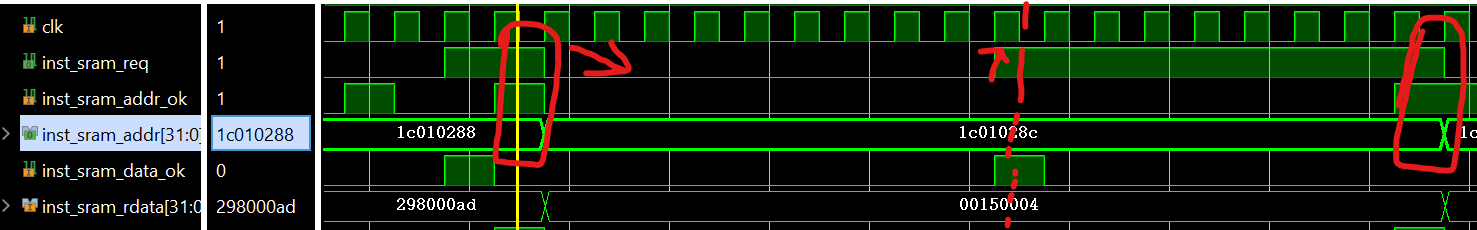
\includegraphics[width=15cm]{fig/fig1.png}
\end{figure}
如时序图中所示,在发送第一个请求后(第一个红色方框),主动拉低 req 信号,等到数据相应握手成功后,立即拉高 req 请求信号,
准备发送新事务的请求。

\item pre\_if级与if级的握手信号

\begin{lstlisting}[language=verilog]
  assign if_allowin       =   ~if_valid 
                            | if_ready_go & id_allowin ;    // if与id级握手成功 
 assign pre_if_readygo   =   pre_if_reqed_reg               // pre_if级已经与sram握手成功
                            |inst_sram_req & inst_sram_addr_ok; // pre_if级刚好与sram握手成功
 assign to_if_valid      =    resetn;  
\end{lstlisting}
\begin{figure}[H]
  \centering
  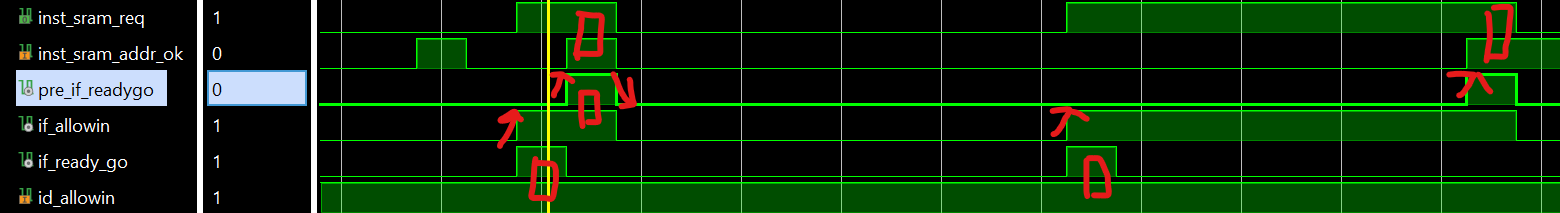
\includegraphics[width=15cm]{fig/fig2.png}
\end{figure}
如时序图所示,在if级与id级完成握手后,立即拉高if的alloin信号。

pre\_if级 的req信号与 \verb|inst_sram_addr_ok|完成握手后,立即拉高pre\_if级的readygo信号。

pre\_if级与if级完成握手后,数据由pre\_if级传递给if级,相应的握手信号在下一个clk双双拉低。

\item 在pre\_if就返回请求的指令,(此时if_allowin = 0)

在pre\_if级设置一个指令缓存,保存这个已经取回但无法进入if级的指令码。


\begin{lstlisting}[language=verilog]
  always @(posedge clk) begin     // pre if 已经发出请求,且没有进入if级
  if(~resetn)                 // 同时可以表明,当前inst_sram返回的指令是属于pre_if级的,而不是if级的
      pre_if_reqed_reg <= 1'b0;
  else if(pre_if_readygo && if_allowin)   // move forward to if
      pre_if_reqed_reg <= 1'b0;
  else if(inst_sram_req && inst_sram_addr_ok) // 握手成功,且不能进入if级
      pre_if_reqed_reg <= 1'b1;
end
always @(posedge clk) begin
  if(~resetn)begin
      pre_if_ir_valid <= 1'b0;
      pre_if_ir <= 32'b0;
  end
  else if(    inst_sram_data_ok    // 指令返回
              & pre_if_reqed_reg  // pre if 已经发出请求,且没有进入if级
              & ~if_allowin       // 不能进入if级
              & ~inst_cancel)     begin   
      pre_if_ir_valid <= 1'b1;
      pre_if_ir <= inst_sram_rdata;
  end
  else if(if_allowin & pre_if_readygo)begin
      pre_if_ir_valid <= 1'b0;
  end
end
\end{lstlisting}
\begin{figure}[H]
  \centering
  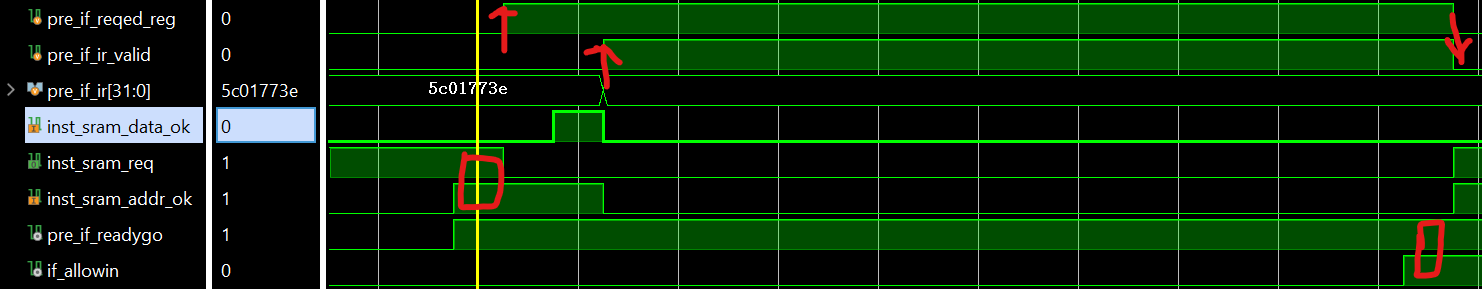
\includegraphics[width=15cm]{fig/fig3.png}
\end{figure}
如图,在pre if 与 sram 地址握手成功后,但是if\_allowin = 0, 不能进入if级,则在下一个clk拉高pre\_if\_reqed\_reg信号,表示
pre if 级当前已经发送了一条请求,且如果此时返回指令,则是对应pre if 级的pc,而不是if级的。

当if级的allowin拉高以后,pre\_if级的指令缓存则传递给if级的指令缓存。


\item if级接受到指令,但是id级还不让进入

与上一个问题一样,在if级同样设置一个指令缓存,来暂存返回的指令。

\item 异常清空流水线

当需要清空流水线时,或者跳转有效时,首先将if和pre\_if级的指令缓存的valid信号置低。

新增一个触发器inst\_cancel,
如果if级或者pre\_if级有已经发出请求,但是没有返回的事务,则将该触发器拉高,等到请求返回后,把他拉低。

并且使用该信号拉低vaild信号。达到丢弃该返回的指令的目的。
\begin{lstlisting}[language=verilog]
  /* 清空流水线时,第一个指令需要丢弃*/
always @(posedge clk) begin
  if(~resetn)
      inst_cancel <= 1'b0;
  else if (   (if_valid & ~if_ir_valid & ~inst_sram_data_ok  // if正在等待指令返回
              |pre_if_reqed_reg & ~inst_sram_data_ok)
          & (flush | br_taken))
      inst_cancel <= 1'b1;
  else if(inst_sram_data_ok)      // 异常后第一个需要被舍弃的指令返回
      inst_cancel <= 1'b0;
end

assign if_to_id_valid   =   if_ready_go & ~inst_cancel;
\end{lstlisting}
\end{enumerate}



\noindent
$\bullet$
\textbf{添加AXI总线支持}。
\vspace{1ex}
\begin{enumerate}
  \item 读请求和读响应
  
  \begin{figure}[H]
    \centering
    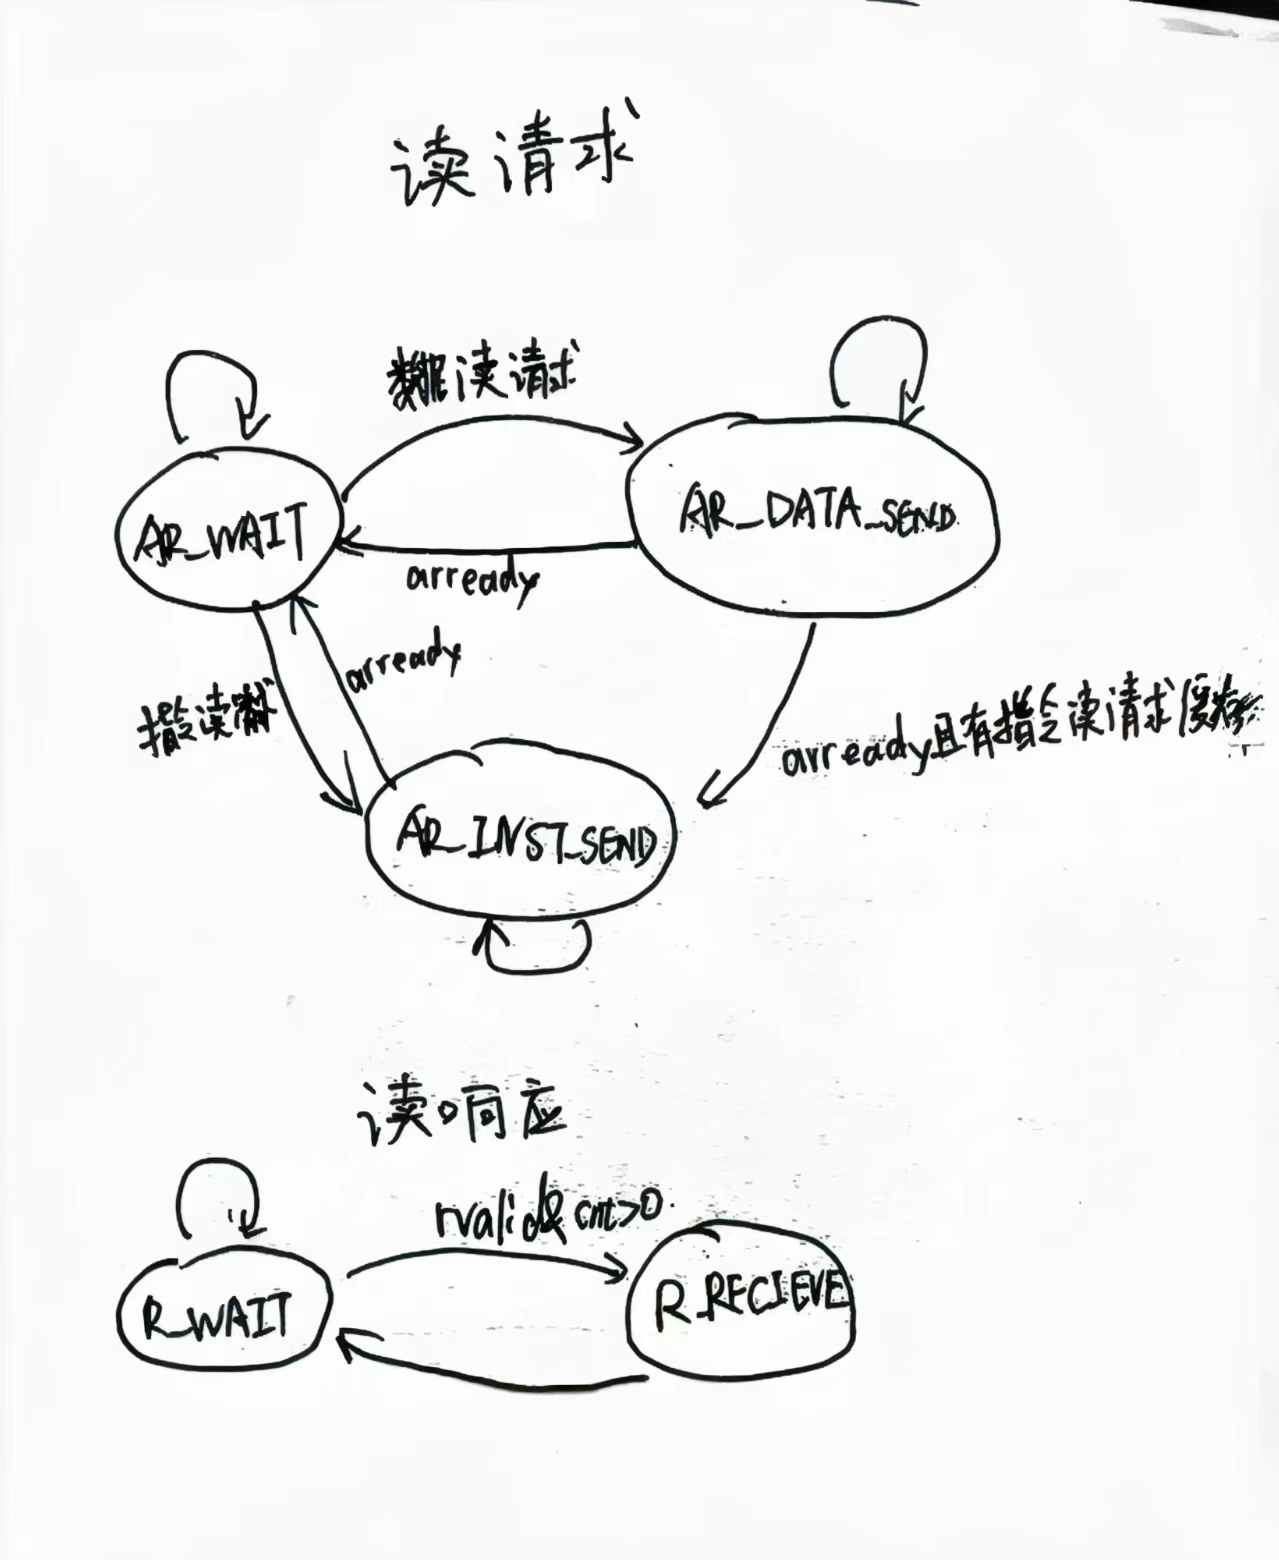
\includegraphics[width=10cm]{fig/fig4.jpg}
  \end{figure}
  分别用两个独立的状态机来控制读请求和读响应通道的行为。
  \begin{enumerate}
    \item 读请求通道
    
    当读请求和写请求状态机都处于wait状态时,拉高两个类SRAM从方的addr\_ok信号,表示可以接受读请求和写请求。

    \begin{lstlisting}
assign inst_sram_addr_ok = ar_current_state == AR_WAIT && aw_current_state == AW_WAIT;
assign data_sram_addr_ok = ar_current_state == AR_WAIT && aw_current_state == AW_WAIT;
    \end{lstlisting}


    如果在AR_WAIT中同时接受到数据读请求和指令读请求,则将指令读请求的地址暂存起来。在AR\_DATA\_SEND阶段将数据读请求的地址握手完成后,再进入AR\_INST\_SEND阶段
    发送指令读请求的地址。

    保证数据端发过来的读请求的优先级固定高于取值端发来的读请求。
  \item 读响应通道
  在R\_WAIT阶段拉高rready,表示可以接受从AXI从端发送的读数据。
  \begin{lstlisting}[language=verilog]
  assign rready = r_current_state == R_WAIT;
  \end{lstlisting}
  当AXI从方将rvalid置为有效,则在下一个clk跳转到R_RECIEVE,将读数据缓存,并根据ID值发给对应的类SRAM主方。
\end{enumerate}
\item 写请求和写响应通道
\begin{figure}[H]
  \centering
  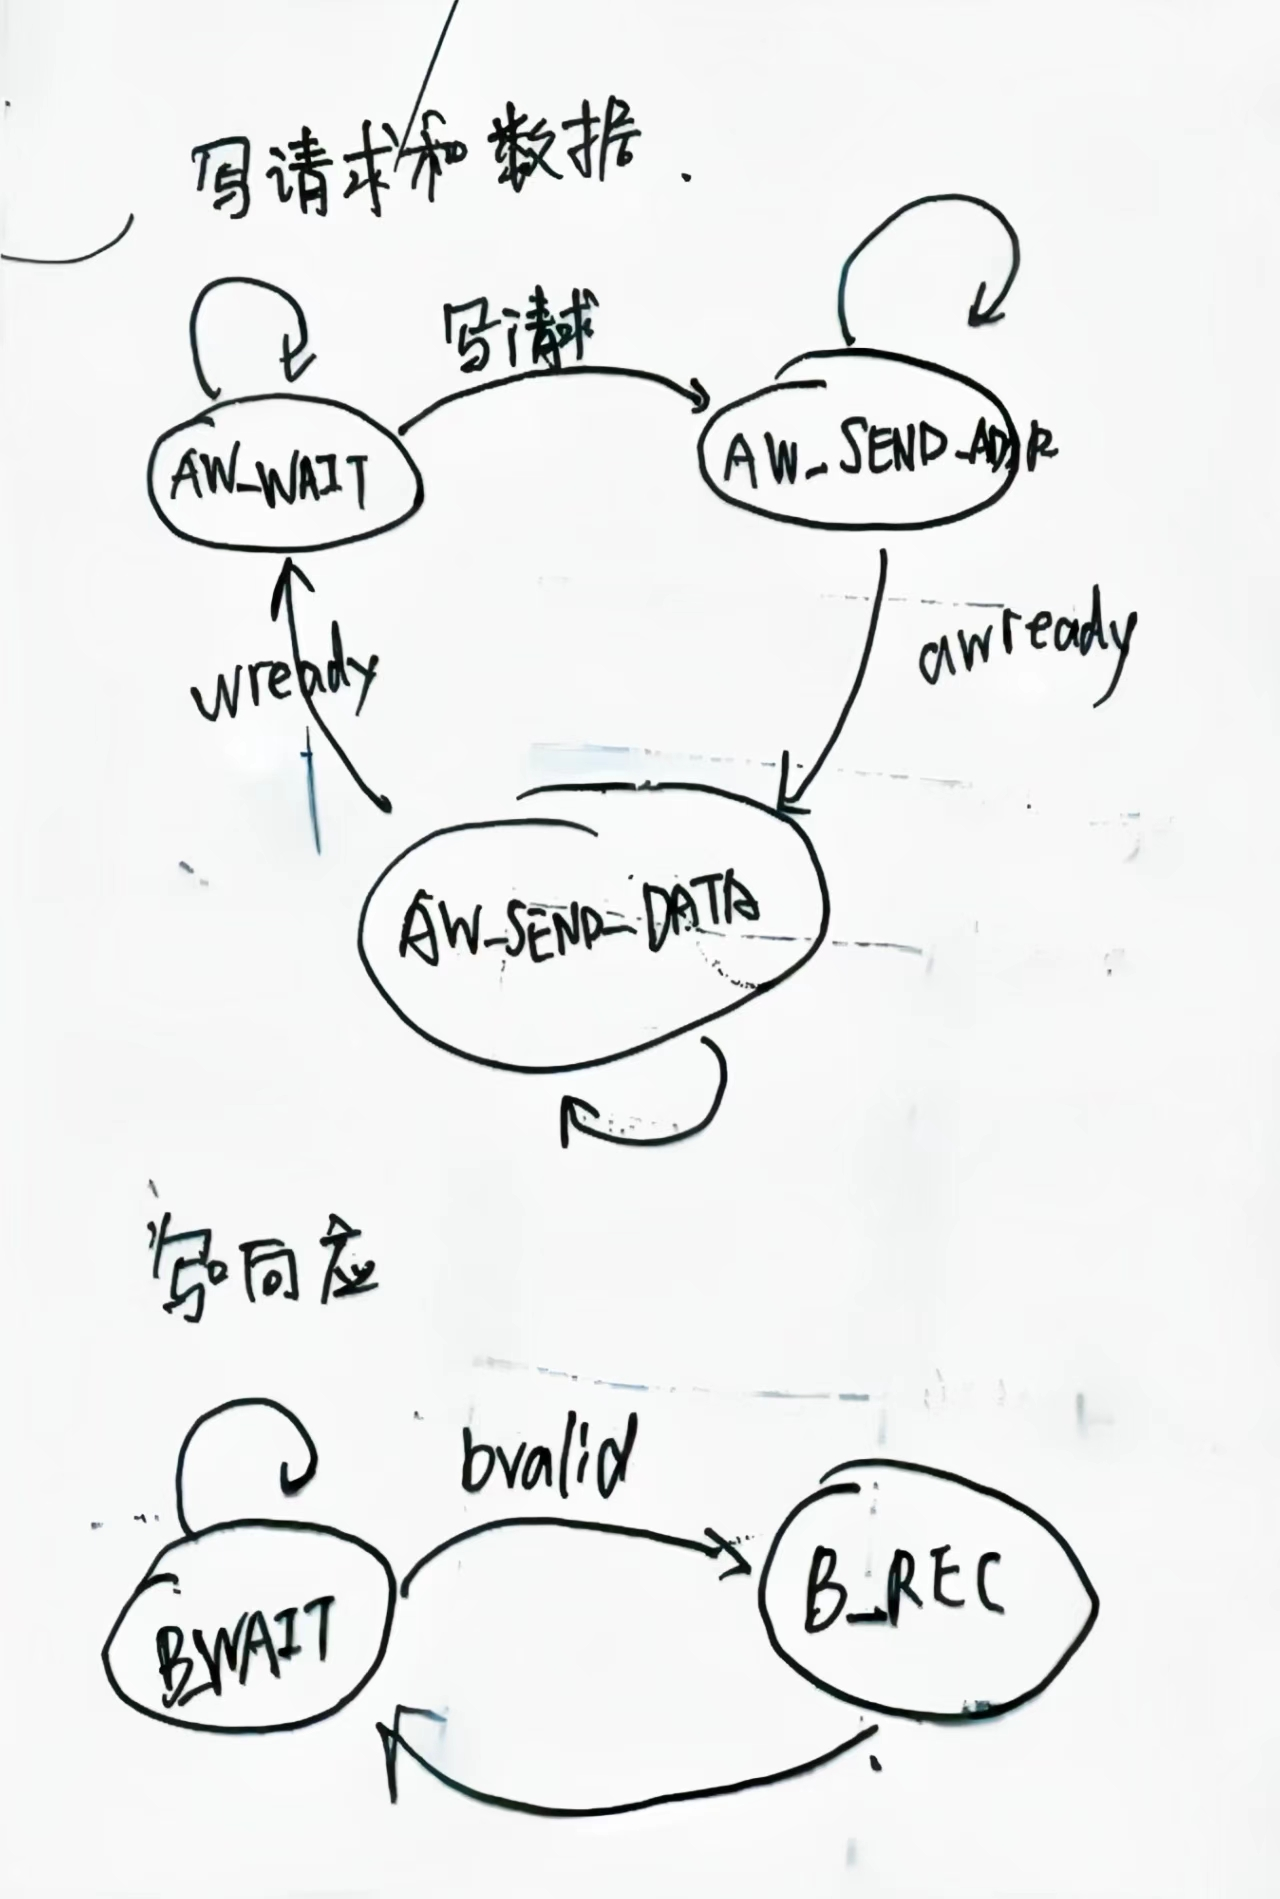
\includegraphics[width=10cm]{fig/fig5.jpg}
\end{figure}
分别用两个独立的状态机来控制写请求和写响应通道的行为。
\begin{enumerate}
  \item 写请求和写数据通道

  在wait阶段接受到写请求后,状态机跳转到SEND\_ADDR阶段发送访存的地址。
  
  在地址发送握手成功后,状态机跳转到SEND\_DATA阶段发送写数据。

  \item 写响应
  
  在wait阶段接受到AXI从方发送的写响应后,状态机跳转到B\_REC状态,向类SRAM总线主方发送\verb|data_sram_data_ok|有效信号

  \begin{lstlisting}[language=verilog]
always @(*)begin
    case (b_current_state)
        B_WAIT:begin
            if(bvalid)
                b_next_state = B_REC;
            else 
                b_next_state <= B_WAIT;
        end
        B_REC:begin
            b_next_state = B_WAIT;
        end
    endcase
end
  \end{lstlisting}
\end{enumerate}

\end{enumerate}





\section{实验过程中遇到的问题、对问题的思考过程及解决方法(比如RTL代码中出现的逻辑bug,逻辑仿真和FPGA调试过程中的难点等)}

\noindent
$\bullet$
\textbf{清空流水线或跳转指令将指令缓存置无效bug}。

当flush或者br\_taken有效时,如果直接在指令缓存更新的代码中,添加在下一排将指令缓存valid置0的代码后,
会出现错误的丢弃跳转后取得第一条指令。

对照波形图排查后发现,是因为在inst\_cancel更新得逻辑中,上述操作只是将指令缓存\verb|if_ir_valid|置为无效,而不将if流水级得有效信号\verb|if_valid|
置低,会导致该逻辑判断if级有已经发送请求但还没有返回指令的事务,则会丢弃接下来接收到的第一条指令。

\begin{lstlisting}[language=verilog]
  /* 清空流水线时,第一个指令需要丢弃*/
  always @(posedge clk) begin
      if(~resetn)
          inst_cancel <= 1'b0;
      else if (   (if_valid & ~if_ir_valid & ~inst_sram_data_ok  // if正在等待指令返回
                  |pre_if_reqed_reg & ~inst_sram_data_ok)     // pre if 正在等待指令返回
              & (flush | br_taken))
          inst_cancel <= 1'b1;
      else if(inst_sram_data_ok)      // 异常后第一个需要被舍弃的指令返回
          inst_cancel <= 1'b0;
  end
\end{lstlisting}

最后,当flush或者br\_taken有效时,不改变\verb|if_ir_valid|的值,而是将id级的allowin拉高,并且将id级的下一排的valid置0,如果if级有指令缓存,
则会在下一个clk传递给id级而消耗掉。
\begin{lstlisting}[language=verilog]
  assign id_allowin       =   ~id_valid 
  | id_ready_go & ex_allowin 
  | br_taken | flush;             // 消耗if级错误指令缓存 
  
  always @(posedge clk) begin
  if(~resetn)
  id_valid <= 1'b0;
  else if(br_taken || flush)  // 发生异常或者跳转时,下一排将id级valid置0
  id_valid <= 1'b0;
  else if(id_allowin)
  id_valid <= if_to_id_valid;
  end
\end{lstlisting}
\noindent
$\bullet$
\textbf{指令译码定义太宽泛导致异常判断出错}。


         

      
\vspace{1ex}

\section{小组成员分工合作情况}
王敬华负责exp13的中断处理和整体的debug工作

李霄宇负责exp13的异常处理和计时器指令的实现

艾华春负责if级取指添加类sram总线支持;类sram-axi转接桥

实验报告为根据每人负责代码的部分,写相应部分的报告。
\end{document}